% !TEX root = ../sethomas_thesis_main.tex
\chapter{Overview of SMA Actuator Design}\label{chap:sma-actuator-design}
\section{Introduction}
In the scope of miniaturisation, creating highly integrated robotic system has become possible with the help of smart materials, notably Shape Memory Alloys (SMA). These alloys, having the highest work density, has made it possible to create miniature artificial muscles that can be integrated into compact and lightweight applications. SMAs have an interesting behaviour which consists of recovery any strain imposed on it when heated above a certain critical temperature threshold, often referred to as the Shape Memory Effect (SME). These alloys exploit the SME to create reversible actuators that are lightweight and compact. This effect is highly non-linear and is dependant on multiple variables, resulting in a highly complex and difficult to model behaviour. Thus, designing and sizing these alloys to create optimised actuators for complex applications is difficult and cumbersome.

In this chapter, an overview of the different implementations of SMA actuators are explored. In the context of different applications, the SMA actuators that are embedded in the different robotic systems are investigated. The traditional design methodology for these actuators are studied and presented in this chapter. The different examples of SMA actuators are used to create a conventional design methodology and the different subsystems of the robotic systems are studied. In this chapter, an in-depth look into the advantages and limitation of the methodology is conducted. In this manner, the conventional design methodology can be adapted into taking a holistic view of the robotic system and create a novel design approach that further promotes the integration of the SMA actuator subsystems into the final robotic system.
% application of sma actuators

\section{Working Principle of SMA Actuators}
Shape Memory Alloys are subclass of smart materials that react to heat. This special brand of material where the can mechanically react with the help of some micro-structural changes when subjected to an external non-mechanical stimulus, in this case, temperature. The shape memory effect that occurs in this alloys occurs due to some phase transformation that happens when heated and cooled around a certain transition temperature. At low temperatures, the material exists in its Martensite (M) phase where the material can be deformed easily. These deformations, similar to plastic deformation, results in the material being permanently deformed at these low temperatures. As the alloy is heated up its transition temperature, the material transforms from the M phase to the Austenite (A) phase, recovering any of the \textit{"permanent"} strain imposed on it at low temperatures. This capacity to recover any strain imposed on it and return back to its original shape is often referred to as the shape memory effect. As the material cools below the transition temperature, the alloy returns back to the M phase, allowing the material to be \textit{"plastically"} deformed once again. The detailed description, along with the analytical and numerical models, is detailed in \cref{chap:sma-model}.

The basic idea behind the implementation of the actuator powered by SMAs is to pair the active material with a biasing element. As stated previously, the SMA element requires a deformation at low temperatures to produce any work when heated to its transition temperature. This implies that for the actuator to behave reversibly and create work cycle, a system is required to deform the SMA at low temperature so as to enable the SMA to produce the actuation when heated. A one-directional SMA actuator is also possible where the SMA is stretched and then heated to revert back to its original shape or constrained to generate an increasing stress based on the applied temperature. These actuators can be used for single actuation application such as deployment mechanisms as shown in the work by \todocite (Mohd Jani 2017 Designing SMA linear actuators). However, in this work, the two-directional SMA actuators are explored and studied. These two-directional actuators require a biasing force as the SMA elements can only in one direction. These linear actuators, thus, require some kind of biasing mechanism that can apply a biasing force in the opposite direction. As shown in the work by \todocite (bellouard), the most common mechanisms used to return the SMA back to its neutral position are bias-springs, dead-weights or another SMA element in an antagonistic configuration as shown in \cref{fig:sma-actuators-diagram}.

\begin{figure}[hbt!]
    \centering
    % !TEX root = ../sethomas_thesis_main.tex
\documentclass[border=1mm,
               class=article
               preview]{standalone}
% \usepackage{tikz}
% \usetikzlibrary{decorations.pathmorphing,patterns}
% trim={<left> <lower> <right> <upper>}

\begin{document}
\begin{tikzpicture}[every node/.style={draw,outer sep=0pt,ultra thick,font=\footnotesize}]
\tikzstyle{sma}=[ultra thick,decorate,decoration={zigzag,pre length=4mm,post length=4mm,segment length=4mm, amplitude=2.5mm}]
\tikzstyle{spring}=[ultra thick,decoration={aspect=0.5,pre length=4mm,post length=4mm,segment length=2mm, amplitude=2.5mm,coil},decorate]
\tikzstyle{ground}=[pattern=north east hatch, hatch distance=3mm, hatch thickness=.5pt, fill,draw=none,minimum width=2mm,minimum height=0.1mm]
% \tikzstyle{ground}=[fill,pattern=north east lines,draw=none,minimum width=2mm,minimum height=0.1mm]
% \tikzstyle{damper}=[thick,decoration={markings,
%   mark connection node=dmp,
%   mark=at position 0.5 with
%   {
%     \node (dmp) [thick,inner sep=0pt,transform shape,rotate=-90,minimum width=15pt,minimum height=3pt,draw=none] {};
%     \draw [thick] ($(dmp.north east)+(2pt,0)$) -- (dmp.south east) -- (dmp.south west) -- ($(dmp.north west)+(2pt,0)$);
%     \draw [thick] ($(dmp.north)+(0,-5pt)$) -- ($(dmp.north)+(0,5pt)$);
% }
%   }, decorate]

    % SMA - Spring
    \node (M) [minimum width=20,minimum height=20] {};
    \node (ground) [ground,anchor=north,yshift=-0.25cm,minimum width=1cm] at (M.south) {};
    \draw[ultra thick] (ground.north east) -- (ground.north west);
    \draw [ultra thick] (M.south west) ++ (0.2cm,-0.125cm) circle (0.1cm)  (M.south east) ++ (-0.2cm,-0.125cm) circle (0.1cm);
    \node (groundL) at (M.east) [ground, xshift=-3cm, rotate=-90, minimum height=0.1mm, minimum width=8mm] {};
    \draw[ultra thick] (groundL.north west) -- (groundL.north east);
    \node (groundR) at (M.west) [ground, xshift=+3cm, rotate=90, minimum height=0.1mm, minimum width=8mm] {};
    \draw[ultra thick] (groundR.north west) -- (groundR.north east);
    \draw[spring, color=mygreen] (M.east) -- node[draw=none, anchor=south, yshift=+4mm] {Bias-Spring} (groundR.north);
    \draw[sma, color=myred] (M.west) -- node[draw=none, anchor=south, yshift=+4mm] {SMA} (groundL.north);

    % SMA - SMA
    \begin{scope}[xshift=7cm]
    \node (M) [minimum width=20,minimum height=20] {};
    \node (ground) [ground,anchor=north,yshift=-0.25cm,minimum width=1cm] at (M.south) {};
    \draw[ultra thick] (ground.north east) -- (ground.north west);
    \draw [ultra thick] (M.south west) ++ (0.2cm,-0.125cm) circle (0.1cm)  (M.south east) ++ (-0.2cm,-0.125cm) circle (0.1cm);
    \node (groundL) at (M.east) [ground, xshift=-3cm, rotate=-90, minimum height=0.1mm, minimum width=8mm] {};
    \draw[ultra thick] (groundL.north west) -- (groundL.north east);
    \node (groundR) at (M.west) [ground, xshift=+3cm, rotate=90, minimum height=0.1mm, minimum width=8mm] {};
    \draw[ultra thick] (groundR.north west) -- (groundR.north east);
    \draw[sma, color=mygreen] (M.east) -- node[draw=none, anchor=south, yshift=+4mm] {Antagonist SMA} (groundR.north);% Ant SMA
    \draw[sma, color=myred] (M.west) -- node[draw=none, anchor=south, yshift=+4mm] {SMA} (groundL.north);
    \end{scope}

    % SMA - Deadweight
    \begin{scope}[xshift=3.5cm, yshift=-2cm]
    \node (M) [minimum width=20,minimum height=20] {};
    \node (ground) [ground,anchor=north,yshift=-0.25cm,minimum width=1cm] at (M.south) {};
    \draw[ultra thick] (ground.north east) -- (ground.north west);
    \draw [ultra thick] (M.south west) ++ (0.2cm,-0.125cm) circle (0.1cm)  (M.south east) ++ (-0.2cm,-0.125cm) circle (0.1cm);
    \node (groundL) at (M.east) [ground, xshift=-3cm, rotate=-90, minimum height=0.1mm, minimum width=8mm] {};
    \draw[ultra thick] (groundL.north west) -- (groundL.north east);
    \node (DW) [minimum width=15,minimum height=15, xshift=+2cm, yshift=-1.5cm, color=mygreen] {$m$};
    \node[draw=none, below=1mm of DW.south, color=mygreen] {Deadweight};
    % Pulley
    \node (intermDW) [right=2.5cm of M.east, above=1cm of DW, draw=none] {};
    \draw[ultra thick] ($(intermDW)-(4mm,3mm)$) circle (4mm);
    \draw[ultra thick, rounded corners=4mm, color=mygreen] (M.east) -| (DW.north);
    \draw[ultra thick,fill] ($(intermDW)-(4mm,3mm)$) circle (0.5mm);
    \draw[ultra thick, fill] ($(intermDW)-(4mm,3mm)$) -- ++(2mm,7mm) -- ++(-4mm,0) -- cycle;
    \draw[sma, color=myred] (M.west) -- node[draw=none, anchor=south, yshift=+4mm] {SMA} (groundL.north);
    \end{scope}

    % \draw [sma] (ground1.north) -- ($(M.south east)!(ground1.north)!(M.south west)$);

\end{tikzpicture}
\end{document}

    % \resizebox{0.7\textwidth}{!}{% !TEX root = ../sethomas_thesis_main.tex
\documentclass[border=1mm,
               class=article
               preview]{standalone}
% \usepackage{tikz}
% \usetikzlibrary{decorations.pathmorphing,patterns}
% trim={<left> <lower> <right> <upper>}

\begin{document}
\begin{tikzpicture}[every node/.style={draw,outer sep=0pt,ultra thick,font=\footnotesize}]
\tikzstyle{sma}=[ultra thick,decorate,decoration={zigzag,pre length=4mm,post length=4mm,segment length=4mm, amplitude=2.5mm}]
\tikzstyle{spring}=[ultra thick,decoration={aspect=0.5,pre length=4mm,post length=4mm,segment length=2mm, amplitude=2.5mm,coil},decorate]
\tikzstyle{ground}=[pattern=north east hatch, hatch distance=3mm, hatch thickness=.5pt, fill,draw=none,minimum width=2mm,minimum height=0.1mm]
% \tikzstyle{ground}=[fill,pattern=north east lines,draw=none,minimum width=2mm,minimum height=0.1mm]
% \tikzstyle{damper}=[thick,decoration={markings,
%   mark connection node=dmp,
%   mark=at position 0.5 with
%   {
%     \node (dmp) [thick,inner sep=0pt,transform shape,rotate=-90,minimum width=15pt,minimum height=3pt,draw=none] {};
%     \draw [thick] ($(dmp.north east)+(2pt,0)$) -- (dmp.south east) -- (dmp.south west) -- ($(dmp.north west)+(2pt,0)$);
%     \draw [thick] ($(dmp.north)+(0,-5pt)$) -- ($(dmp.north)+(0,5pt)$);
% }
%   }, decorate]

    % SMA - Spring
    \node (M) [minimum width=20,minimum height=20] {};
    \node (ground) [ground,anchor=north,yshift=-0.25cm,minimum width=1cm] at (M.south) {};
    \draw[ultra thick] (ground.north east) -- (ground.north west);
    \draw [ultra thick] (M.south west) ++ (0.2cm,-0.125cm) circle (0.1cm)  (M.south east) ++ (-0.2cm,-0.125cm) circle (0.1cm);
    \node (groundL) at (M.east) [ground, xshift=-3cm, rotate=-90, minimum height=0.1mm, minimum width=8mm] {};
    \draw[ultra thick] (groundL.north west) -- (groundL.north east);
    \node (groundR) at (M.west) [ground, xshift=+3cm, rotate=90, minimum height=0.1mm, minimum width=8mm] {};
    \draw[ultra thick] (groundR.north west) -- (groundR.north east);
    \draw[spring, color=mygreen] (M.east) -- node[draw=none, anchor=south, yshift=+4mm] {Bias-Spring} (groundR.north);
    \draw[sma, color=myred] (M.west) -- node[draw=none, anchor=south, yshift=+4mm] {SMA} (groundL.north);

    % SMA - SMA
    \begin{scope}[xshift=7cm]
    \node (M) [minimum width=20,minimum height=20] {};
    \node (ground) [ground,anchor=north,yshift=-0.25cm,minimum width=1cm] at (M.south) {};
    \draw[ultra thick] (ground.north east) -- (ground.north west);
    \draw [ultra thick] (M.south west) ++ (0.2cm,-0.125cm) circle (0.1cm)  (M.south east) ++ (-0.2cm,-0.125cm) circle (0.1cm);
    \node (groundL) at (M.east) [ground, xshift=-3cm, rotate=-90, minimum height=0.1mm, minimum width=8mm] {};
    \draw[ultra thick] (groundL.north west) -- (groundL.north east);
    \node (groundR) at (M.west) [ground, xshift=+3cm, rotate=90, minimum height=0.1mm, minimum width=8mm] {};
    \draw[ultra thick] (groundR.north west) -- (groundR.north east);
    \draw[sma, color=mygreen] (M.east) -- node[draw=none, anchor=south, yshift=+4mm] {Antagonist SMA} (groundR.north);% Ant SMA
    \draw[sma, color=myred] (M.west) -- node[draw=none, anchor=south, yshift=+4mm] {SMA} (groundL.north);
    \end{scope}

    % SMA - Deadweight
    \begin{scope}[xshift=3.5cm, yshift=-2cm]
    \node (M) [minimum width=20,minimum height=20] {};
    \node (ground) [ground,anchor=north,yshift=-0.25cm,minimum width=1cm] at (M.south) {};
    \draw[ultra thick] (ground.north east) -- (ground.north west);
    \draw [ultra thick] (M.south west) ++ (0.2cm,-0.125cm) circle (0.1cm)  (M.south east) ++ (-0.2cm,-0.125cm) circle (0.1cm);
    \node (groundL) at (M.east) [ground, xshift=-3cm, rotate=-90, minimum height=0.1mm, minimum width=8mm] {};
    \draw[ultra thick] (groundL.north west) -- (groundL.north east);
    \node (DW) [minimum width=15,minimum height=15, xshift=+2cm, yshift=-1.5cm, color=mygreen] {$m$};
    \node[draw=none, below=1mm of DW.south, color=mygreen] {Deadweight};
    % Pulley
    \node (intermDW) [right=2.5cm of M.east, above=1cm of DW, draw=none] {};
    \draw[ultra thick] ($(intermDW)-(4mm,3mm)$) circle (4mm);
    \draw[ultra thick, rounded corners=4mm, color=mygreen] (M.east) -| (DW.north);
    \draw[ultra thick,fill] ($(intermDW)-(4mm,3mm)$) circle (0.5mm);
    \draw[ultra thick, fill] ($(intermDW)-(4mm,3mm)$) -- ++(2mm,7mm) -- ++(-4mm,0) -- cycle;
    \draw[sma, color=myred] (M.west) -- node[draw=none, anchor=south, yshift=+4mm] {SMA} (groundL.north);
    \end{scope}

    % \draw [sma] (ground1.north) -- ($(M.south east)!(ground1.north)!(M.south west)$);

\end{tikzpicture}
\end{document}
}
    \caption{A schematic representation of the basic types of linear SMA actuators. In general, a separate kinematic stage is used to transform the linear output into the desired output.}
    \label{fig:sma-actuators-diagram}
\end{figure}
The \textbf{Biased-Deadweight SMA Actuator} has the advantage of being quite simple to implement as it consists of simply applying a constant load to the active element irrespective of the temperature. Here, the SMA based on the phase will displace the constant load by a fixed stroke. At low temperatures, the deadweight elongates the SMA element and as the SMA heats up and changes phase, the load will be displaced. As there is always the same constant load, there is a high risk of overheating the SMA and risking reaching stresses above the recommended maximum pull force of the SMA. Thus, to prevent this irreversible damage to the SMA actuator, a constant load that is below the maximum pull force of the SMA is used. This greatly limits the maximum load that can be displaced by the SMA actuator preventing widespread adoption of this method of implementation.

The \textbf{Biased-Spring SMA Actuator}, on the other hand, consists of pairing the SMA element with a biasing passive spring. This method of implementation is also quite simple to implement and thus, is the most widely used method for designing SMA actuators. Here, the idea consists of using a passive spring to apply a spring force to the SMA at low temperatures. This allows the SMA to be deformed and activates the SME when the alloy is heated. As the material transforms from the M to the A phase, the spring is deformed while the SMA element returns to its original shape. Here, due to the increasing elongation of the spring, an increasing spring force acts on the SMA as the temperature is increased. This implies that based on the temperature and the rigidity of the spring, the force and stroke of the actuator can be sized. The sizing methodology and analytical models of this type of actuator will be detailed in \cref{chap:sma-model}. However, the actuator can only be controlled in one direction during the heating phase, while during the cooling, the SMA actuator returns back to its neutral position uncontrolled.


The \textbf{Antagonistic SMA Actuator} consists of pairing the SMA element with an antagonistic biasing SMA element. In this method, the actuator can be actuated in both directions. As the first SMA is heated, the strain recovery cause the antagonistic SMA to be deformed and elongated. When heating the antagonistic SMA, the inverse effect occurs, where the first SMA is deformed and elongated while the antagonistic SMA reverts back to its original shape. Thus, by alternatively heating the SMA pair, the actuator can be made to actuate in both directions. The primary downside to such an implementation is the difficulty in sizing and controlling such an actuator due to the compounding of the highly non-linear nature of each of the SMAs. These SMAs are still widely used in many applications do to the additional degree of freedom. The sizing methodology of these actuators will be described in \cref{chap:sma-model}.

The three methods of implementation represent the majority of the different types of SMA actuators. Using this biasing principle for pre-stretching the SMA element, a reversible and cyclical actuator can be fabricated. It is important to note that the biasing element along with the SMA represent only the subsystems that create the reversible work offered by the active material. However, when creating an SMA actuator, additional structure and elements are required to form a complete actuator for the required application.

\section{Analysis of SMA Actuators}
As stated previously, the principal advantage of actuators powered by SMAs are the fact that, owing to their high work density, these actuators can be designed to be compact and lightweight. However, this is only the case when designed specifically for the required application. Due to the active nature of the material, when the SME is exploited specifically for the requirements of the use case, the resulting actuator can be integrated into the overall robotic application. Thus, when analysing the various methods in which these SMA actuators are designed, it is important to consider the application and its domain. Due to the long cycling time of the SMA elements, SMA actuators are primarily used in systems and domains where low bandwidth but compact actuators are required. Based on the work by \todocite (Mohd Jani, 2014) and \todocite (sreekumar, 2007), these actuators have been used in automotive as miniaturised actuators for various subsystems to replace traditional electromagnetic or pneumatic actuators. In aerospace applications, where there are geometric volume constraints, they have been used to create micro-grippers, vibration dampers or deployment mechanisms. Furthermore, due to their bio-compatibility, these SMA actuators have also found its way into the biomedical field where they have been used to create miniature medical and surgical instruments such as endoscopes, medical tweezers and stents among others. Recently, however, there has been wide interest in creating miniature bio-inspired and reconfigurable robots where these SMAs are used as artificial muscles. Thus, in this section, the goal is to explore the various domains in which SMA actuators are employed and study, using some examples, the different design parameters and choices used to create appropriate actuators for the appropriate application. By doing so, the important and key factors that make up the design of SMA actuators can be established. These factors can, thus, be used to detail the various ares in which these actuators can be improved and optimised such that when designing future SMA actuators, the final systems can be further integrated. By exploring the design choice used in the following examples, a design methodology can be established for creating novel improved SMA actuators.

% Biomedical
\subsection{Biomedical Applications}
Due to the tight volume constraints in the biomedical field, actuators that prioritize compact footprints have been favoured. Furthermore, in the medical field, reduced noise, vibration, and contamination are necessary. A high time response is not required and slower actuation can be tolerated. This makes it an ideal domain for SMA actuators to flourish. The choice of the examples presented in this section is to examine various types of SMA actuators implemented in the biomedical field to extrapolate the various design parameters and choices used for this specific application.

In the first example, the authors, \cite{liuMesoscaleShapeMemory2019}, have a developed a mesoscale actuator used to maintain the visual clarity of the lens in endoscopes during invasive robotic surgeries as shown in \cref{fig:biomed-examples}(a). Here the main design criteria were the limitation of contaminants and the extreme volume constraints. The actuator must fit on the end of the tip of the endoscope which is inserted within the body during surgery. The tight footprint required for the project specifications has created a need for smart materials, specifically shape memory alloys, to be used in this application. The alloy being biocompatible has also played a key role in the choice of smart material. The actuator, proposed in this work, consists of a simple bias-spring SMA actuator where the active element consists of a thin SMA wire and the biasing element consists of a passive tractional spring. Here, the actuator, using a pin as a simple pivot, transforms the linear motion of the SMA actuator into a rotation of the lens cover. This cover, considered the output, is used to clear the surgical camera maintain the visual clarity during the surgery.
\begin{figure}[hbt!]
    \centering
    % !TEX root = ../../sethomas_thesis_main.tex
\documentclass[border=1mm,
               class=article
               preview]{standalone}
\usepackage{tikz}
% trim={<left> <lower> <right> <upper>}
\begin{document}
\begin{tikzpicture}
    \node[anchor=south west,inner sep=0] (graph) at (0,0) {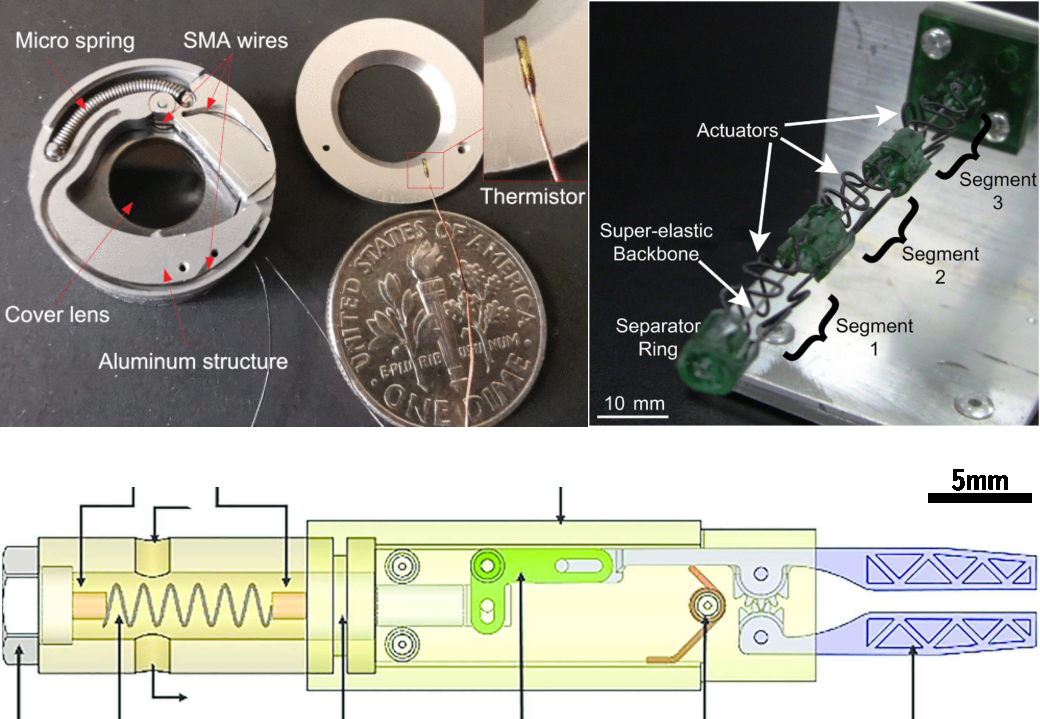
\includegraphics[width=0.7\textwidth]{images/chap1/biomed-examples.pdf}};
    \begin{scope}[x={(graph.south east)},y={(graph.north west)}]
    \node (a) at (0.04,0.46) {\color{white}\textbf{(a)}};
    \node (b) at (0.6,0.95) {\color{white}\textbf{(b)}};
    \node (c) at (0.04,0.37) {\textbf{(c)}};

    \node at (0.02,-0.05) {\footnotesize \makecell[c]{End\\nut}};
    \node at (0.12,-0.05) {\footnotesize \makecell[c]{SMA\\spring}};
    \node at (0.33,-0.02) {\footnotesize Piston};
    \node at (0.5,-0.02) {\footnotesize Link};
    \node at (0.67,-0.05) {\footnotesize \makecell[c]{Steel torsional\\spring}};
    \node at (0.87,-0.05) {\footnotesize \makecell[c]{Gripper\\jaws}};
    \node at (0.17,0.35) {\footnotesize Mount};
    \node at (0.54,0.35) {\footnotesize Base};
    \end{scope}
\end{tikzpicture}
\end{document}

    \caption{Examples of different implementations of SMA actuators in the biomedical field : (a) An SMA powered actuator used for visual clarity in Surgical cameras taken from the work by \cite{liuMesoscaleShapeMemory2019} (b) A multi-segmented SMA endoscope taken from the work by \cite{abdulkadirMultisegmentedShapeMemory2019b} (c) A minimally invasive surgical gripper taken from the work by \cite{roshanDesignFabricationMinimally2018}}
    \label{fig:biomed-examples}
\end{figure}

In the work by \cite{abdulkadirMultisegmentedShapeMemory2019b}, the authors have designed and fabricated a multi-segmented SMA-based actuator system for endoscopic applications as shown in \cref{fig:biomed-examples}(b). In this second example, the main design criteria were the volume constraints of the actuator, the biocompatibility of the actuator and the high strokes required. As with the previous example, the actuator is used in minimally invasive surgery and thus requires the actuator to be biocompatible and prevent any unwanted pollution of the body during operation. Further, due to the tight volume constraints of the human body, the actuator makes use of the high volumetric work density of the alloy to create this compact actuator. The actuator proposed in this work consists of multiple bias-spring SMA actuators arranged in an antagonistic manner. Here, a flat SMA spring is used to provide the high strokes required and is paired with an elastic backbone that provides the rigidity for the endoscope while also allowing the SMA spring to return back to its original state during cooling. Opposing SMA flat spring are placed surrounding the biasing element to allow the endoscope to actuate in other directions and increase the degrees of freedom.

In this last example, the authors, \cite{roshanDesignFabricationMinimally2018}, have designed and fabricated a minimally invasive surgical gripper based on an SMA spring actuator. As stated by the authors, in minimally invasive surgeries, manipulations are often performed in confined and tight spaces and thus, the main design criteria were the miniaturisation of the actuator and maintaining the high energy density of the alloy. In this example, the proposed gripper is fabricated using several components including an SMA spring as the active element and torsional spring as a biasing element as shown in \cref{fig:biomed-examples}(c). Furthermore, a pivot linking system is used as a kinematic stage that converts the linear actuation of the SMA spring into a rotational output of the gripper jaws.

In the case of actuators designed for biomedical applications, there is a large focus for compact and work dense actuators. Furthermore, in some cases, the biocompatibility of the SMA plays a large role in the choice of the actuator. The design of the final actuator in this application is largely dependant on the volume constraints imposed by the human body. Here, actuators generally tend to value stroke over force output and thus, SMA springs are generally used as they come with higher elongations but at the price of lower force outputs. Using bias-spring SMA actuators allows the actuator to have a reversible and cyclical actuation. In the presented examples, the bias-spring was chosen over the antagonistic SMA due to the reduced complexity and simplicity in the control. The implementation of sensors and control electronics can often result in increase volume requirements and can degrade the work density of the final system.

% Automotive / Aerospace
\subsection{Automotive and Aerospace Applications}
As in the case of SMAs in the biomedical field, the high work density and the ability of SMA actuators to be compact and lightweight has allowed them to be attractive in the automotive and aerospace field. A common requirement of automotive products are high miniaturisation and integration. The small size and weight of SMA actuators has made them ideal in aerospace applications. In this section, some examples have been studied to determine the various design requirements of SMA actuators in this field. By studying the various types of automotive or aerospace SMA actuators, the various design criteria and limitations can be extracted.

\begin{figure}[hbt!]
    \centering
    % !TEX root = ../../sethomas_thesis_main.tex
\documentclass[border=1mm,
               class=article
               preview]{standalone}
\usepackage{tikz}
% trim={<left> <lower> <right> <upper>}
\begin{document}
\begin{tikzpicture}
    \node[anchor=south west,inner sep=0] (graph) at (0,0) {
        \begin{annotationimage}{trim={0 0cm 0 0cm},clip, width=0.75\textwidth}{images/chap1/auto-examples.pdf}
         \draw[annotation left = {\makecell[r]{SMA\\wire} at 0.7}] to (0.235,0.7);
         \draw[annotation left = {Bias-spring at 0.79}] to (0.24,0.79);
         \draw[annotation left = {Mirror at 0.9}] to (0.1,0.9);
         \draw[annotation right = {\makecell[l]{SMA\\coil} at 0.79}] to (0.74,0.79);
         \draw[annotation right = {\makecell[l]{Power\\electronics} at 0.9}] to (0.7,0.9);
         \draw[annotation right = {Output at 0.7}] to (0.95,0.75);
         \draw[coordinate label = {\color{white}\textbf{(a)} at (0.03,0.96)}];
         \draw[coordinate label = {\color{white}\textbf{(b)} at (0.4,0.96)}];
         \draw[coordinate label = {\color{black}\textbf{(c)} at (0.03,0.56)}];
       \end{annotationimage}};
    % \begin{scope}[x={(graph.south east)},y={(graph.north west)}]
    % \node (a) at (0.14,0.97) {\color{white}\textbf{(a)}};
    % \node (b) at (0.43,0.97) {\color{white}\textbf{(b)}};
    % \node (c) at (0.14,0.56) {\textbf{(c)}};
    % \end{scope}
\end{tikzpicture}
\end{document}

    \caption{Examples of different implementations of SMA actuators in automotive and aerospace applications : (a) An active SMA powered mirror taken from the work by \cite{williamsControlAutomotiveShape2010a} (b) An automotive tumble flap powered by an SMA actuator taken from the work by \cite{belliniMechatronicDesignShape2009} (c) An active span-wise adaptive wing taken from the work by \cite{belliniMechatronicDesignShape2009}}
    \label{fig:auto-examples}
\end{figure}

In the first example, the authors, \cite{williamsControlAutomotiveShape2010a}, have designed and fabricated a lightweight and cost effective active mirror actuator as shown in \cref{fig:auto-examples}(a). The traditional power mirrors that use electromechanical actuators have been commonplace in the automotive industry. The authors have designed an alternative using SMAs to create an active automobile power mirror that is lightweight and work dense actuator. In this work, the active mirror consists of a biasing spring surrounded by four SMA wires. The mirror, mounted on a spherical joint, can be actuated in the four cardinal directions. Since a limited stroke length is required, SMA wires have been used to actuate the mirror. Furthermore, a single passive spring has been implemented as a biasing element for each of the SMA wire actuators. The spherical pivot on which the mirror is mounted converts the linear movement of the SMA actuator into the required rotational movement. The SMA wires are actuated using Joule's heating by passing a current across the wires. The control of the actuator is performed by using a variable structure controller. The authors have focused their work to be lightweight and robust and thus have used the high work density of the alloy to their advantage.

In the second example, the authors, \cite{belliniMechatronicDesignShape2009}, have sized and fabricated a binary SMA actuator for automotive tumble flaps. Here, this solid-state actuation system is developed to replace the existing traditional electromagnetic and pneumatic actuators used in the industry. In this work, the authors focused on creating a miniature actuator by harnessing the high work density of the shape memory alloy. The main constraints presented in this work, as stated by the author, are the power to weight ratio, robustness and reliability of the actuators. Furthermore, the clean, silent and smooth operation of the actuator in addition to its self-sensing capabilities added to the attractive nature of the material in this application. In this prototype, the basic concept consists of using SMA coils with an antagonistic SMA coil as the biasing element as shown in \cref{fig:auto-examples}(b). Furthermore, in the work, a thermoelectric module is used to aid in the heat transfer from one SMA coil to the other for increased operation frequency. Here, a pair of SMA coils are used in parallel to increase the overall force output of the actuator.

In this final example, the authors, \cite{benafanRecentAdvancementsRotary2019a}, have integrated an SMA actuator within the wing of aircraft to create an active span-wise adaptive wing as shown in \cref{fig:auto-examples}(c). In the aerospace domain, creating lightweight actuators that can reduce the load for aircrafts is the primary constraint that have allowed SMAs to penetrate the industry. The high work density of the materials allows for the creation of lightweight actuators that can still produce the large forces required in this application as displayed in this work. SMA actuators can be utilized to build safer, lighter, and less complicated systems that are compatible with future electric-aircraft concepts. In this work, a bias-spring rotational SMA actuator is created to alter the shape of the wing. A SMA tube is paired with a torsional bias spring to create the rotation actuator. Position sensors and a heating cartridge is integrated into the system to create the full working prototype for the adaptive wing. Due to the low profile of the structure and by using an SMA tube, the entire actuator fits withing the profile of the wing while still delivering high output forces.

As shown in these examples, the high force output and the ability to create lightweight systems has been the primary design criteria that has allowed SMA actuator to proliferate in this engineering domain. In each example, the high work density of the SMA has been exploited to create actuators that can produce large force while remaining compact and lightweight. In each example, discrete systems were used to create the active and biasing elements. A separate conversion mechanism employing hinges or pivots were used in each case to convert the output of the SMA actuator into the required motions showing an area in which some degrading of the work density is present.

% Industrial
\subsection{Industrial Applications}
% Intro to industrial application
The primary reason that SMAs have started to be integrated into industrial applications has been the need for lightweight and powerful actuators. The high power and energy densities of the SMA has made it an ideal candidate to save weight and construction space when compared to traditional electric and pneumatic actuators. Furthermore, these SMA industrial actuators operate with reduced noise and emissions with is often overlooked in industrial applications but can be essential in clean-room applications. In this section, various examples of industrial gripper powered by shape memory alloys are presented so as to understand an establish a clearer picture of the various design requirements and constraints present in the domain.

\begin{figure}[h]
    \centering
    % !TEX root = ../../sethomas_thesis_main.tex
\documentclass[border=1mm,
               class=article
               preview]{standalone}
\usepackage{tikz}
% trim={<left> <lower> <right> <upper>}
\begin{document}
\begin{tikzpicture}
    \node[anchor=south west,inner sep=0] (graph) at (0,0) {
        \begin{annotationimage}{trim={0 0cm 0 0cm},clip, width=0.9\textwidth}{images/chap1/industrial-examples-v2.pdf}
        % Gripper annotations
        \draw[coordinate label = {\color{black}{\normalfont\tiny{SMA linear actuator}} at (0.565,0.536)}];
        \draw[coordinate label = {\color{black}\normalfont\scriptsize{\makecell[r]{Gripper\\jaw}} at (0.58,0.27)}];
        \draw[coordinate label = {\color{black}\normalfont\scriptsize{\makecell[c]{Cross-shear\\kinematic stage}} at (0.805,0.29)}];
        % Suction annotations
        \draw[coordinate label = {\color{black}\normalfont\scriptsize{Spring adjustment screws} at (0.13,0.525)}];
         \draw[coordinate label = {\color{black}\normalfont\scriptsize{Membrane adjustment} at (0.14,0.47)}];
         \draw[coordinate label = {\color{black}\normalfont\scriptsize{Upper SMA fixation} at (0.16,0.41)}];
         \draw[coordinate label = {\color{black}\normalfont\scriptsize{Bias-spring} at (0.194,0.355)}];
         \draw[coordinate label = {\color{black}\normalfont\scriptsize{SMA wire} at (0.205,0.29)}];
         \draw[coordinate label = {\color{black}\normalfont\scriptsize{Electrical contacts} at (0.165,0.23)}];
         \draw[coordinate label = {\color{black}\normalfont\scriptsize{Lower SMA fixation} at (0.16,0.15)}];

         \draw[coordinate label = {\color{white}\textbf{(a)} at (0.03,0.59)}];
         \draw[coordinate label = {\color{black}\textbf{(b)} at (0.445,0.035)}];
         \draw[coordinate label = {\color{black}\textbf{(c)} at (0.98,0.035)}];
       \end{annotationimage}};
\end{tikzpicture}
\end{document}

    \caption{Examples of different implementations of SMA actuators in industrial applications : (a) A soft robotic gripper powered by an SMA wire taken from the work by \cite{rodrigueCurvedShapeMemory2017a} (b) A bistable vacuum gripper taken from the work by \cite{motzkiEnergyefficientSMAVacuum2016} (c) A two-prong industrial robotic powered an SMA wire taken from the work by \cite{luNovelDesignParallel2019}}
    \label{fig:industrial-examples}
\end{figure}

In the first example, the authors, \cite{rodrigueCurvedShapeMemory2017a}, have designed and fabricated a soft robotic gripper powered by an SMA wire. Here, the SMA wire-based soft bending actuator was designed so as to exploit the power-to-weight ratio of the material to create a lightweight robotic finger as shown in \cref{fig:industrial-examples}(a). In the work, the proposed actuator consists of a curved polydimethylsiloxane (PDMS) matrix with an embedded SMA wire. Here, the wire, acting as the active element, is biased by the PDMS matrix. During the activation, the SMA wire attempts to straighten itself when heated and is reverted back to its curved state by the PDMS matrix during cooling. The high power-to-weight ratio allows three $200~\mu$m SMA wires to exert $1.5$ N of gripping force. The use of the biasing PDMS matrix allows the repeated actuation of the actuator. The curved nature of the PDMS matrix and the actuator acts as the kinematic stage that converts the actuation of the SMA into the required gripping motion. In this work, the authors have prioritized creating an actuator that is lightweight and has soft actuation to not damage the grasped object. The use of SMAs in this application has allowed the authors to create a lightweight actuator while still enabling a high grasping force.

In this second case study, the authors, \cite{motzkiEnergyefficientSMAVacuum2016}, have developed an SMA-powered vacuum gripper. The gripper, as shown in \cref{fig:industrial-examples}(b), consists of a bias-spring surrounded by a long SMA wire in traction. Here, the SMA wire is wound around multiple screws to create the illusion of multiple independent SMA wires that work in parallel to increase the output forces. Furthermore, a bistable mechanism is used to convert the SMA actuation into a constant holding force that require no additional energy from the SMA after the initial trigger force. The gripper is actuated using Joule's heating by passing a current across the SMA wire and the authors have implement a resistance measurement and self-sensing capability for the control of the gripper. In this work, the leading design criteria was the energy efficiency of the bistable mechanism and the high output forces of the SMA wire. The SMA wire system allowed the final vacuum gripper to be lightweight while still offering the required forces to trigger the snap-through of the bistable mechanism.

In the final example, the authors, \cite{luNovelDesignParallel2019}, have designed and fabricated a robotic gripper which aims to grasp to uncooperative objects as shown in \cref{fig:industrial-examples}(c). In this work, the authors have chosen to replace traditional hydraulic actuators with an SMA-powered actuator due to their reduced complexity and points of failure and their high energy density, low energy consumption and quick response. The robotic gripper consists of three major subsystems: the SMA linear actuator, the hinge coupler mechanism and the gripping claws. The SMA linear actuator consists of a eight SMA wires fixed on one end and fixed to a sliding shaft on the other end. This allows a stroke amplification of the linear actuator without reducing the output forces. The system offers some redundancy where if one of the wires fails, the other wires allows the continued operation of the SMA gripper. The coupler mechanism makes use of cross-shear hinge mechanism to convert the linear actuator of the SMA actuator into the required dual motion of the claws. The mechanism also offers a stroke amplification to the overall actuator. The biasing element allows the repeated actuation of the system and is accomplished using a simple passive spring. In this work, the authors have prioritized the high work density of the alloy to create a compact system with higher energy efficiency and higher longevity.

As shown in the presented examples, the key design criteria of SMA actuators in industrial applications are the lightweight and compact nature of the resulting SMA actuators. The use of SMAs and their high power-to-weight ratio has allowed actuators to be created that are lightweight and are, thus, highly attractive as end-effectors for robotic arms. Furthermore, using bistable mechanisms and bias springs has allowed SMA-powered industrial grippers to be energy efficient by not requiring continuous energy to grasp objects. The biasing elements also allow the repeated actuation of the gripper without introducing any contaminants or complex assemblies. The slow cooling time and the reduce operating frequency has always been a challenge in industrial applications but has been outweighed by the high work density of the alloy.

% Bio-inspired
\subsection{Bio-inspired Robotic Applications}
In the hunt for creating bio-inspired robotic system, there has been a intentional effort to finding smart materials that have similar performances to biological muscles. In this regards, the high volumetric work density of SMAs and its naturally compliant natures has made it comparable to biological muscles and has made it a primary candidate for bio-inspired applications. When creating bio-inspired robotic systems, the primary design constraints are often the weight and volume of the system. SMAs, being the primary candidate for lightweight systems, allows robotic systems to be highly integrated and make use of the energy density of the material. Implementing traditional electromagnetic and pneumatic systems can be useful in creating tethered systems but when designing untethered systems that have a focus on reduced weight have been forced to implement SMA-powered actuators.

\begin{figure}[hbt!]
    \centering
    % !TEX root = ../../sethomas_thesis_main.tex
\documentclass[border=1mm,
               class=article
               preview]{standalone}
\usepackage{tikz}
% trim={<left> <lower> <right> <upper>}

\begin{document}
\begin{tikzpicture}
    \node[anchor=south west,inner sep=0] (graph) at (0,0) {
        \begin{annotationimage}{trim={0 0cm 0 0cm},clip, width=0.9\textwidth}{images/chap1/bio-examples.pdf}
         \draw[coordinate label = {\color{white}\normalfont\tiny{$10$ mm} at (0.68,0.05)}];

         \draw[coordinate label = {\color{black}\textbf{(a)} at (0.03,0.98)}];
         \draw[coordinate label = {\color{black}\textbf{(b)} at (0.98,0.98)}];
         \draw[coordinate label = {\color{white}\textbf{(c)} at (0.27,0.37)}];
       \end{annotationimage}};
      \begin{scope}[x={(graph.south east)},y={(graph.north west)}]
          \node (SMA) at (0.28,0.705) {};
          \node (SMAtext) at (0.28,0.56) {\tiny SMA Coil};
          \draw[latex-] (SMA) -- (SMAtext);
      \end{scope}
\end{tikzpicture}
\end{document}

    \caption{Examples of different implementations of SMA actuators in industrial applications : (a) A soft-actuated crawling robot taken from the work by \cite{liangShapeMemoryAlloy2020} (b) A highly dynamic mobile robot taken from the work by \cite{huangHighlyDynamicShape2019} (c) A sub-milligram crawling SMA-powered robot taken from the work by \cite{yang88milligramInsectscaleAutonomous2020a}}
    \label{fig:bio-examples}
\end{figure}

In this first example, the authors, \cite{liangShapeMemoryAlloy2020}, have designed an SMA-actuated soft crawling robot. In this work, the authors have focused on creating a lightweight actuator that is able to propel itself across a surface with a gait similar to an inchworm as shown in \cref{fig:bio-examples}(a). Due to the tight volume and weight constrains of the application, the authors have incorporated the elastic nature of the robot body as the biasing element to the SMA coil. However, the robot requires a passive spring as an auxiliary biasing element to accelerate the robot recovery and improve the gait coordination of the insect robot. The slow cooling of the SMA coil results in a slow gait for the insect robot but reducing the diameter of the coil can drastically increase the robot speed. However, the control of the robot and the electronics have not been integrated into the system. This tethered crawling robot has exploited the high energy density of the SMA to create a small lightweight robot.

In the second example, the work by \cite{huangHighlyDynamicShape2019}, presents a highly dynamic SMA-powered moving robot. Here, as shown in \cref{fig:bio-examples}(b), the authors exploit the naturally compliant nature and the high work density of the alloy to create the actuator that powered the moving robot. In this work, the SMA actuator consists of a single SMA wire encased in a biasing silicone elastomer. Furthermore, a thermally conductive elastomer is used to dissipate the heat from the SMA, acting as a heat sink, to increase the time response of the robot. Miniaturised power electronics has been added to the robot to allow the robot to move untethered. The flexural response of the SMA wire is used to actuate the robot and is also used as the crawling motion. The authors, by creating a highly integrated system, has allowed them to fully exploit the high work density of the smart material.

In the last example, the authors, \cite{yang88milligramInsectscaleAutonomous2020a}, have developed an ultra-lightweight crawling robot that is powered by a shape memory alloy wire. This autonomous sub-gram micro-robot, as shown in \cref{fig:bio-examples}(c), makes use a thin SMA wire attached to a small hinge that allows the actuation of the legs when the SMA is heated. The biasing element in this case is composed of a thin leaf spring that is used to create the two-way activation of the SMA actuator. The authors have achieved such a lightweight SMA-powered robot by avoiding the use of any senors or electronics with the use a chemical heating element. A reservoir of methanol is used to heat the SMA wire using vents that are opened and closed based on the position of the robot legs. This mechanical control has allowed the authors to fully harness the high work density of the SMA wire and create an ultra-lightweight robot. In this case, the primary design principle that motivated the design of the robot was the final weight and energy density of the system.

When considering the different examples of bio-inspired robotic system, the main design criteria considered by the different authors has been to reduce the overall weight and complexity of the system. When creating such miniature and lightweight systems, designing monolithic parts with reduced complexity and assembly has been critical in harnessing the work density of the SMA actuator. In these examples, the SMA actuator has been integrated into the body of the robot as opposed to separating the actuator and robot body into discrete subsystems.

\section{Design Criteria}
The various actuators shown in the previous section displays the diversity and variety of designs that exist to create an SMA actuator. When considering the domains in which SMAs are used shows that these alloys have become an attraction option to replace traditional pneumatic and electromagnetic actuators. Furthermore, the domain in which the SMA is used has a large impact on the design and implementation of the actuator. This implies that when designing SMA-powered actuators, a holistic approach must be taken where the application and the entire system is considered.

In the case of biomedical applications, the SMA actuators are implemented based on the design constraints imposed by the human body. The various examples of biomedical applications are summarised in \cref{tab:biomed-subsystems-examples}. In this domain, the fact that SMA actuators have smooth operation and do not introduce any particulate matter makes them an attraction alternative. Furthermore, when dealing with the tight volume constraints imposed by the human body, the high work density of the material becomes a crucial detail in the choice of active material. Furthermore, as the SMA can be heated rapidly, using Joule's heating which involves simply passing a current across the SMA, a rapid actuation can be obtained which is highly attractive in this domain. As shown in the examples, small and powerful SMA wires and springs are used to create the actuators while passive micro-springs are employed to enable two-way actuation.

\begin{table}[hbt]
    \centering
    \caption{A summary of the various implementations of the biomedical SMA actuators.}
    % !TEX root = ../../sethomas_thesis_main.tex
\documentclass[border=1mm,
               class=article
               preview]{standalone}

\begin{document}
\renewcommand{\arraystretch}{1.5}
 {\footnotesize\rowcolors{1}{black!5}{black!10}
% \begin{tabular}{lccccc}
% \begin{tabular}{p{3cm}P{1.25cm}P{1.25cm}P{1.5cm}P{1.5cm}P{1.5cm}}
% \begin{tabular}{p{2cm}P{2cm}P{2cm}P{2cm}P{2cm}P{2cm}}
\begin{tabular}{p{0.18\textwidth-2\tabcolsep}
                p{0.15\textwidth-2\tabcolsep}
                p{0.16\textwidth-2\tabcolsep}
                p{0.16\textwidth-2\tabcolsep}
                p{0.16\textwidth-2\tabcolsep}
                p{0.18\textwidth-2\tabcolsep}}
   \rowcolor{black}  & \textbf{\color{white} \parbox[t]{1.5cm}{Active\\Element}} & \textbf{\color{white} \parbox[t]{1.5cm}{Biasing\\Element}} & \textbf{\color{white} Kinematic Stage} & \textbf{\color{white} \parbox[t]{1.5cm}{Heating\\Strategy}} & \textbf{\color{white} Sensor}\\
   \cite{liuMesoscaleShapeMemory2019} & Wire & Micro-spring & Pin Pivot & Joule's heating & Thermistor\\
   \cite{abdulkadirMultisegmentedShapeMemory2019b} & Flat springs & Elastic backbone & Rigid link / Backbone & Joule's heating & External Camera\\
   \cite{roshanDesignFabricationMinimally2018} & Spring & Torsional spring & Pins and gears & Heated water & Thermocouple\\
\end{tabular}}
\renewcommand{\arraystretch}{1}
\end{document}

    \label{tab:biomed-subsystems-examples}
\end{table}

When it comes to SMA actuators designed for automotive and aerospace applications, they are often conceived with high force outputs as a priority. Since the shape memory effect is scalable, these alloys can be used in micro and macro applications. Here, traditionally actuators used in this field at this scale tend to be bulky and heavy. The high work density of the alloy allows creating powerful actuators with large force outputs that are still lightweight when compared to similar traditional actuators. Furthermore, the rapid actuation and the low bandwidth required in these application has also allowed SMAs to penetrate the market. The fact that, often, SMA-powered actuators have a simple design and reduce complexity allowing these actuators to be used in this domain that values longer lifespan and reduced failure points. In \cref{tab:auto-subsystems-examples}, the implementation summary of the different examples are shown.

\begin{table}[hbt]
    \centering
    \caption{A summary of the various implementations of the aerospace and automotive SMA actuators from the different examples.}
    % !TEX root = ../../sethomas_thesis_main.tex
\documentclass[border=1mm,
               class=article
               preview]{standalone}

\begin{document}
\renewcommand{\arraystretch}{1.5}
 {\footnotesize\rowcolors{1}{black!5}{black!10}
% \begin{tabular}{p{2cm}P{2cm}P{2cm}P{2cm}P{2cm}P{2cm}}
\begin{tabular}{p{0.17\textwidth-2\tabcolsep}
                p{0.15\textwidth-2\tabcolsep}
                p{0.16\textwidth-2\tabcolsep}
                p{0.16\textwidth-2\tabcolsep}
                p{0.16\textwidth-2\tabcolsep}
                p{0.18\textwidth-2\tabcolsep}}
   \rowcolor{black}  & \textbf{\color{white} \parbox[t]{1.5cm}{Active\\Element}} & \textbf{\color{white} \parbox[t]{1.5cm}{Biasing\\Element}} & \textbf{\color{white} Kinematic Stage} & \textbf{\color{white} \parbox[t]{1.5cm}{Heating\\Strategy}} & \textbf{\color{white} Sensor}\\
   \cite{williamsControlAutomotiveShape2010a} & Wires (in parallel) & Spring & Pivot & Joule's heating & External position sensor\\
   \cite{belliniMechatronicDesignShape2009} & Springs (in parallel) & Antagonistic SMA springs & Linear guide & Thermo-electric module & None\\
   \cite{benafanRecentAdvancementsRotary2019a} & Tube & Torsional spring & Bearing and hinges & Heater catridge & Thermocouple\\
\end{tabular}}
\renewcommand{\arraystretch}{1}
\end{document}

    \label{tab:auto-subsystems-examples}
\end{table}

However in industrial applications, the requirement to higher operating bandwidth has often limited the use of SMAs. In cases where a soft gripper or a gripper that is lightweight, the natural compliance and the work density of the material has allowed it to adapt to the requirements of the industry. In some cases, the absence of contaminant as in the case of pneumatic grippers can be an attractive characteristic that force the adoption of SMA-based grippers. In this domain, the weight and force outputs of the actuator are the primary design constraints when considering the choice of active material. When designing SMA-powered grippers for industrial application, the weight if often factored into the design process. Furthermore, as the primary challenge of SMA actuators is the low operating bandwith due to the cooling requirements, adequate sizing must be considered when designing the active SMA element for the use case scenario. In \cref{tab:industrial-subsystems-examples}, a summary of the different implementation strategies are shown when creating such SMA-based industrial grippers.

\begin{table}[hbt]
    \centering
    \caption{A summary of the various implementations of the industrial SMA actuators.}
    % !TEX root = ../../sethomas_thesis_main.tex
\documentclass[border=1mm,
               class=article
               preview]{standalone}

\begin{document}
\renewcommand{\arraystretch}{1.5}
 {\footnotesize\rowcolors{1}{black!5}{black!10}
% \begin{tabular}{p{2cm}P{2cm}P{2cm}P{2cm}P{2cm}P{2cm}}
\begin{tabular}{p{0.17\textwidth-2\tabcolsep}
                p{0.14\textwidth-2\tabcolsep}
                p{0.17\textwidth-2\tabcolsep}
                p{0.16\textwidth-2\tabcolsep}
                p{0.16\textwidth-2\tabcolsep}
                p{0.18\textwidth-2\tabcolsep}}
   \rowcolor{black}  & \textbf{\color{white} \parbox[t]{1.5cm}{Active\\Element}} & \textbf{\color{white} \parbox[t]{1.5cm}{Biasing\\Element}} & \textbf{\color{white} Kinematic Stage} & \textbf{\color{white} \parbox[t]{1.5cm}{Heating\\Strategy}} & \textbf{\color{white} Sensor}\\
   \cite{rodrigueCurvedShapeMemory2017a} & Wire & PDMS matrix & Shape setting & Joule's heating & None\\
   \cite{motzkiEnergyefficientSMAVacuum2016} & Wire & Spring & Bistable mechanism & Joule's heating & None\\
   \cite{luNovelDesignParallel2019} & Wires (in series) & Spring & Cross-shear coupler & Joule's heating & External position sensor\\
\end{tabular}}
\renewcommand{\arraystretch}{1}
\end{document}

    \label{tab:industrial-subsystems-examples}
\end{table}

In the last major domain in which SMAs are often employed, they are favoured due to their resemblance to human muscles with respect to their volumetric work density. In the case of bio-inspired actuators, the goal has always been to create the smallest and lightest actuator such that the system can remain in the mesoscale. This often imposed a strict weight and volume constraint for the actuator when dealing with bio-inspired robotic systems. SMAs have often been the first choice for such system as creating lightweight actuators are its speciality. In \cref{tab:bioinspired-subsystems-examples}, the different implementations are displayed for the previously presented examples. Often, these robotic systems have been designed around the material rather than the other way around. This holistic approach, often used in this domain, is rarely exploited in the other applications. The tight weight and volume constraints have force the authors to create highly integrated systems.

\begin{table}[hbt]
    \centering
    \caption{A summary of the various implementations of the bio-inspired SMA-powered systems.}
    % !TEX root = ../../sethomas_thesis_main.tex
\documentclass[border=1mm,
               class=article
               preview]{standalone}

\begin{document}
\renewcommand{\arraystretch}{1.5}
 {\footnotesize\rowcolors{1}{black!5}{black!10}
% \begin{tabular}{p{2cm}P{2cm}P{2cm}P{2cm}P{2cm}P{2cm}}
\begin{tabular}{@{}p{0.20\textwidth-2\tabcolsep}
                p{0.14\textwidth-2\tabcolsep}
                p{0.17\textwidth-2\tabcolsep}
                p{0.16\textwidth-2\tabcolsep}
                p{0.17\textwidth-2\tabcolsep}
                p{0.14\textwidth-2\tabcolsep}@{}}
   \rowcolor{black}  & \textbf{\color{white} \parbox[t]{1.5cm}{Active\\Element}} & \textbf{\color{white} \parbox[t]{1.5cm}{Biasing\\Element}} & \textbf{\color{white} Kinematic Stage} & \textbf{\color{white} \parbox[t]{1.5cm}{Heating\\Strategy}} & \textbf{\color{white} Sensor}\\
   \cite{liangShapeMemoryAlloy2020} & Spring & Elastic body and bias spring & Elastic body geometry & Joule's heating & None\\
   \cite{huangHighlyDynamicShape2019} & Wire & Silcome elastomer matrix & Elastomer shape setting & Joule's heating (Heatsink) & Thermistor\\
   \cite{yang88milligramInsectscaleAutonomous2020a} & Wire & Leaf spring & Flexural hinge & Chemical heating & Mechanical vents\\
\end{tabular}}
\renewcommand{\arraystretch}{1}
\end{document}

    \label{tab:bioinspired-subsystems-examples}
\end{table}

% Summary of the design criteria of SMA actuators
As observed with the various examples, the constraints of the application plays a major role in the implementation and design of the SMA actuator. When studying the different applications, the major design constraints that are considered when designing these SMA-powered actuators, include :
\begin{itemize}
    \item a weight constraint
    \item a volume constraint
    \item a high force or stroke output requirement
    \item a reduce contaminants or biocompatibility requirement
    \item a rapid actuation requirement
    \item or a two-way actuation requirement
\end{itemize}
Using these design constraints, the sizing and design choices can be made to create an SMA-powered actuator that is more suited for the desired application. In this work, these constraints and lessons learned from the various examples in the different applications are exploited and translated to other situations.

\section{Traditional Design Elements of an SMA-based System}
Using the various examples of SMA actuators, that were explored in the previous section, a holistic approach to SMA actuator design can be taken. In each case, the primary goal of the actuator was to exploit the high work density of the smart material to create a lightweight or compact actuator. Often, sub-optimal solutions were employed when compared with the implementations in other domains. In the case of bio-inspired systems, the SMA actuators had a large focus on the work density and the final weight of the system, however, in other domains such as industrial applications, these techniques could be employed to further improve the performances of the grippers. By translating lessons learned from one domain to another, the hope is to allow the entire robotic system to fully harness the high work density of the SMAs.

With the goal of improving the work density of the final system, the different SMA-powered examples can be studied to establish the areas in which a more integrated approach can be taken. As shown in the previous section, there are common subsystems that exist when designing the SMA-based robotic system. By establishing a commonality between the different types of actuators, the strategies employed in one domain can be easily translated to another. As shown in \cref{fig:hexahon-base-layer}, the SMA actuator can be divided to four different basic building blocks. These subsystems each have a specific role and allows the SMA actuator perform the require output when actuated using a thermal load.

% Building blocks figure
\begin{figure}[hbt] % t for top of the page, H could be put to impose the position of the float
  \centering
  \begin{tikzpicture}
    \node[anchor=south west,inner sep=0] (graph) at (0,0) {
\includegraphics[trim={0 0 0 0},clip, width=0.8\textwidth]{images/chap1/hexgon-base-layer.pdf}};
	% Insert a relative reference based on image dimensions
    \begin{scope}[x={(graph.south east)},y={(graph.north west)}]
    \node[] at (0.19, 0.5) {\textcolor{white}{\large Active Element}};
    \node[] at (0.5, 0.75) {\textcolor{white}{\large Kinematic Stage}};
    \node[] at (0.5, 0.24) {\textcolor{white}{\large Control Stage}};
    \node[] at (0.81, 0.5) {\textcolor{white}{\large Biasing Element}};
    \end{scope}
    \end{tikzpicture}
  \caption{A visual representation of the different subsystems that exist in the traditional SMA-based systems.}
  \label{fig:hexahon-base-layer}
\end{figure}

% Basic tradition subsystems of SMA actuators
\subsection{Building Blocks of an SMA Actuator}
Often, these different subsystems exists as discrete building blocks in the SMA-based robotic system. These subsystems each fulfil a different role in the operation of the SMA actuator.

The \textbf{Active Element} is the SMA element that is present within the system and is responsible to providing the work for actuation. The SMA, as shown in the examples, can be fabricated in various shapes. Often, they are used as wires when space is limited, low strokes and high force outputs are required. When higher strokes are required, SMA coils are used as they are able to elongate over 100\% of their length with a trade-off in force output. In certain cases, thin SMA sheets are used for higher force output. In most cases, however, as passive cooling is employed, the geometry of the SMA element plays a major role in the operating frequency of the actuator. Here, thinner and smaller SMA sheets or wires allow for faster time responses.

In applications where two-way or repeatable activation is required, the \textbf{Biasing Element} is added to the actuator. The role of the biasing element consists of deforming the SMA at low temperatures so that the shape memory effect can occur when the active element is heated. As mentioned previously, the most simple forms of biasing elements consist of a deadweight, a passive spring or an antagonistic SMA. These elements allow the actuator to be actuated repeatedly or in both directions. The dependence of the SMA actuator for such a biasing subsystem greatly degrades the work density of the SMA actuator when considered as a whole. Often, in the case of SMA actuators, these passive elements allow the repeated actuation of the active element without adding any additional work.

As the traditional SMA-based actuator is often a linear actuation, some kind of \textbf{Kinematic Stage} is present to convert the linear movement of the actuator into the required output motion. In most cases, such as grippers, the simple linear motion of the SMA actuator is not sufficient. In such cases, the kinematic stage is employed using pins, hinges, gears and bearings, to convert the linear motion of the actuator into a more complex motion. In certain cases, this stage is used to amplify the stroke or output forces of the actuator. In the most simple applications, a hinge or lever arm is used to convert the linear rotation of the actuator into a rotational one. The kinematic stage is, often, a critical subsystem when designing an SMA-powered robotics system.

The last subsystem, the \textbf{Control Stage}, consists of the electronics, sensors or heating mechanism used to active and control the shape memory effect. In the case of SMAs, a thermal load must be applied to the active material to activate the shape memory effect and initiate the strain recovery of the alloy. In most cases, the simplest solution consists of harnessing the internal resistance of the SMA and heat the alloy using Joule's heating. Here, a current is passed across the SMA to allow Joule's losses to heat the material above its transition temperature and produce the required stroke. In such a case, considerable care must be taken to not overheat the material which will results in permanent shape setting of the SMA or destruction of the SMA wire or coil. In such cases, a temperature sensor, position sensor or even sensorless control is employed to control the heating process of the active element. This additional stage consisting of sensors or control electronics is not considered in the work density of the actuator and often degrades the density and efficiency. In cases where space or weight is limited, the control stage is an expensive addition to the actuator.
% with examples of types of implementations of each subsystem
\section{Summary and Conclusion}
In this chapter, the working principle of the traditional SMA-powered actuator and the various examples of different implementations of SMA actuators in literature is presented. In the case of SMAs, the material requires a biasing element when requiring two-way activation. Only when the alloy is pre-stressed above a critical stress will the material show any strain recovery when heated. Thus, in this chapter, the most common types of SMA actuator implementations are presented, detailing the ways in which the alloy can be pre-stressed as shown in the work by \todocite (bellouard). Using passive springs or an antagonistic SMA as the biasing element is often the simplest and more efficient solution to creating a two-way SMA actuator.

In an effort to understand the different design considerations that exists when conceiving and fabricating SMA-based robotic systems, this chapter explores the major domains in which SMA-powered actuators thrive. Due to the high work density of the alloy, this material is often found in applications where weight and space constraints exist such as the biomedical, aerospace or automotive, industrial and bio-inspired applications. By studying various examples in each case, the dependence of the domain on the design constraints and implementations was made evident. Each major domain has a set of their own constraints which heavily affect the implementation of the actuator.

By studying these examples, a set of design considerations and constraints can be extracted so as to create a primary design principle when design SMA-powered actuators. In most cases, the work density of the alloy is the primary reason that compels the authors to integrate the SMA into their robotic system. When considering the various applications, taking a holistic design approach where the entire robotic system including the constraints are considered, can result in a considerable optimization of the work density. By exploring the strategies employed in certain domains and translating them to other domains can result in novel actuators.

Furthermore, in this chapter, studying the robotic systems in the major fields has been used to establish the different subsystems that exists in a traditional SMA-powered actuators. The four subsystems are shown to have their respective functions and constraints. They are often designed independent of each other and are implemented without the consideration of the other subsystems. These building blocks of the SMA actuator, being discrete systems, show a considerable area in which these designs can be improved. Having discrete subsystems, that do not take into account the other subsystems, degrade the work density of the final system. In this work, a novel holistic approach to designing integrated SMA-powered actuators will be presented.

When designing such systems, sizing the SMA element based on the surrounding components is essential. The interactions between the different subsystems is often a balancing act that requires careful consideration of their respective mechanical properties. In the following chapter, the different SMA models are detailed and presented so as to adequately size the SMA element for the required stroke and force output of the actuator. The shape memory effect of the alloy is a multi-physical behaviour that is non-linear. The following chapter will present a simplified model and sizing methodology to create an adapted SMA-powered actuator.
